%%%%%%%%%%%%%%%%%%%%%%%%%%%%%%%%%%%%%%%%%%%%%%%%%%%%%%%%%%%%%%%%%%%%%%%%%%%%%%%%
%
% \file       main.tex
% \brief      Главный файл настроек TeX проекта
% \date       18.05.22 - создан
% \author     Соболев А.А.
%
%%%%%%%%%%%%%%%%%%%%%%%%%%%%%%%%%%%%%%%%%%%%%%%%%%%%%%%%%%%%%%%%%%%%%%%%%%%%%%%%
\documentclass[exampletask]{espd}
%\usepackage[russian]{babel} % polyglossia
\usepackage{setspace}
\usepackage{fontspec}
\usepackage{cite} % Для цитирования
\usepackage{amsmath}
\usepackage{gensymb} % Для знака градуса
\usepackage{mathtools}
\usepackage{listings} % Для листингов исходного кода
\usepackage{hhline} % Для двойной линии отчерка в заголовках таблиц
\usepackage{color} % Цвет для листингов
%\usepackage{inputenc}
%\usepackage{fontenc}
%\usepackage{fancyvrb}

\graphicspath{ {./иллюстрации/} }

\bibliographystyle{gost2008}
\setmainfont{Times New Roman}
%%%%%%%%%%%%%%%%%%%%%%%%%%%%%%%%%%%%%%%%%%%%%%%%%%%%%%%%%%%%%%%%%%%%%%%%%%%%%%%%
% Переопределение команд дефиса
%%%%%%%%%%%%%%%%%%%%%%%%%%%%%%%%%%%%%%%%%%%%%%%%%%%%%%%%%%%%%%%%%%%%%%%%%%%%%%%%
\newcommand{\sdash}{\nobreakdash-}  % Дефис неразрывный без пробелов до и после
\newcommand{\ndash}{\nobreakdash~--~}  % Короткое тире неразрывное с пробелами до и после
\newcommand{\mdash}{\nobreakdash~---~} % Длинное тире неразрывное с пробелами до и после
%%%%%%%%%%%%%%%%%%%%%%%%%%%%%%%%%%%%%%%%%%%%%%%%%%%%%%%%%%%%%%%%%%%%%%%%%%%%%%%%
% Для таблиц longtable
%%%%%%%%%%%%%%%%%%%%%%%%%%%%%%%%%%%%%%%%%%%%%%%%%%%%%%%%%%%%%%%%%%%%%%%%%%%%%%%%
\setlength{\doublerulesep}{1.5pt}% Разделитель между двойным отчерком заголовка таблицы
\floatsetup[longtable]{LTcapwidth=table} % Выравнивание заголовка по левому краю
%%%%%%%%%%%%%%%%%%%%%%%%%%%%%%%%%%%%%%%%%%%%%%%%%%%%%%%%%%%%%%%%%%%%%%%%%%%%%%%%
% Определение форматирования исходного кода в тексте документа
%%%%%%%%%%%%%%%%%%%%%%%%%%%%%%%%%%%%%%%%%%%%%%%%%%%%%%%%%%%%%%%%%%%%%%%%%%%%%%%%
% Можно выделять исходники цветом, но зачем
%\definecolor{dkgreen}{rgb}{0,0.5,0}
%\definecolor{gray}{rgb}{0.5,0.5,0.5}
%\definecolor{mauve}{rgb}{0.58,0,0.82}
\lstset{
	frame=none,
	language=C++,
	aboveskip=3mm,
	belowskip=3mm,
	showstringspaces=false,
	columns=fixed, %flexible,
	basicstyle=\listingtextsize\fontspec{Noto Sans Mono},%{Courier New},
	extendedchars=true, % без символа \ !!! - так поддерживается русский язык в комментариях
	inputencoding=utf8x,
%    escapechar=|,
	numbers=left,
%	numberstyle=\tiny,
%	stepnumber=1,
%	numberstyle=\tiny\color{mauve},
%	keywordstyle=\color{blue},
%	commentstyle=\color{dkgreen},
%	stringstyle=\color{mauve},
	breaklines=true,
	breakatwhitespace=true,
	tabsize=3
}
% Поддержка русского языка в комментариях к исходному коду
\makeatletter % see https://tex.stackexchange.com/a/320345
\lst@InputCatcodes
\def\lst@DefEC{%
	\lst@CCECUse \lst@ProcessLetter
	^^80^^81^^82^^83^^84^^85^^86^^87^^88^^89^^8a^^8b^^8c^^8d^^8e^^8f%
	^^90^^91^^92^^93^^94^^95^^96^^97^^98^^99^^9a^^9b^^9c^^9d^^9e^^9f%
	^^a0^^a1^^a2^^a3^^a4^^a5^^a6^^a7^^a8^^a9^^aa^^ab^^ac^^ad^^ae^^af%
	^^b0^^b1^^b2^^b3^^b4^^b5^^b6^^b7^^b8^^b9^^ba^^bb^^bc^^bd^^be^^bf%
	^^c0^^c1^^c2^^c3^^c4^^c5^^c6^^c7^^c8^^c9^^ca^^cb^^cc^^cd^^ce^^cf%
	^^d0^^d1^^d2^^d3^^d4^^d5^^d6^^d7^^d8^^d9^^da^^db^^dc^^dd^^de^^df%
	^^e0^^e1^^e2^^e3^^e4^^e5^^e6^^e7^^e8^^e9^^ea^^eb^^ec^^ed^^ee^^ef%
	^^f0^^f1^^f2^^f3^^f4^^f5^^f6^^f7^^f8^^f9^^fa^^fb^^fc^^fd^^fe^^ff%
	^^^^20ac^^^^0153^^^^0152%
	% Basic Cyrillic alphabet coverage
	^^^^0410^^^^0411^^^^0412^^^^0413^^^^0414^^^^0415^^^^0416^^^^0417%
	^^^^0418^^^^0419^^^^041a^^^^041b^^^^041c^^^^041d^^^^041e^^^^041f%
	^^^^0420^^^^0421^^^^0422^^^^0423^^^^0424^^^^0425^^^^0426^^^^0427%
	^^^^0428^^^^0429^^^^042a^^^^042b^^^^042c^^^^042d^^^^042e^^^^042f%
	^^^^0430^^^^0431^^^^0432^^^^0433^^^^0434^^^^0435^^^^0436^^^^0437%
	^^^^0438^^^^0439^^^^043a^^^^043b^^^^043c^^^^043d^^^^043e^^^^043f%
	^^^^0440^^^^0441^^^^0442^^^^0443^^^^0444^^^^0445^^^^0446^^^^0447%
	^^^^0448^^^^0449^^^^044a^^^^044b^^^^044c^^^^044d^^^^044e^^^^044f%
	^^^^0401^^^^0451^^^^0020%
	%%%
	^^00}
\lst@RestoreCatcodes
\makeatother
%%%%%%%%%%%%%%%%%%%%%%%%%%%%%%%%%%%%%%%%%%%%%%%%%%%%%%%%%%%%%%%%%%%%%%%%%%%%%%%%%
%% Задание перечислений буквами
%%%%%%%%%%%%%%%%%%%%%%%%%%%%%%%%%%%%%%%%%%%%%%%%%%%%%%%%%%%%%%%%%%%%%%%%%%%%%%%%%
%\usepackage{enumitem}
%
%\makeatletter
%\newcommand{\realasbuk}[1]{\expandafter\russian@realalph\csname c@#1\endcsname}
%
%\def\russian@realAlph#1{\ifcase#1\or
%	А\or Б\or В\or Г\or Д\or Е\or Ж\or
%	З\or И\or К\or Л\or М\or Н\or О\or
%	П\or Р\or С\or Т\or У\or Ф\or Х\or
%	Ц\or Ч\or Ш\or Щ\or Э\or Ю\or Я\else\xpg@ill@value{#1}{russian@Alph}\fi}
%\def\russian@realalph#1{\ifcase#1\or
%	а\or б\or в\or г\or д\or е\or ж\or
%	з\or и\or к\or л\or м\or н\or о\or
%	п\or р\or с\or т\or у\or ф\or х\or
%	ц\or ч\or ш\or щ\or э\or ю\or я\else\xpg@ill@value{#1}{russian@alph}\fi}
%
%\AddEnumerateCounter{\realasbuk}{\russian@realalph}{щ}
%\makeatother
%%%%%%%%%%%%%%%%%%%%%%%%%%%%%%%%%%%%%%%%%%%%%%%%%%%%%%%%%%%%%%%%%%%%%%%%%%%%%%%%
% Задание полей титульных страниц
%%%%%%%%%%%%%%%%%%%%%%%%%%%%%%%%%%%%%%%%%%%%%%%%%%%%%%%%%%%%%%%%%%%%%%%%%%%%%%%%
\newcommand{\productcipher}{АБВГД.12345} % Шифр изделия

\firstapplication{\productcipher} % Первое применение
\referencenumber{\productcipher} % Справ №

\organizationcode{01234} % Код организации
\registrationcode{56789} % Регистрационный код
\redaction{01} % Номер редакции
\documentnumber{03} % Номер документа данного вида
%\partnumber{1} % Номер части документа - чтобы задать - надо фиксить класс espd

% СОГЛАСОВАНО
\customerrank{Начальник\\межгалактической комиссии}
\customername{А.Б.~Заказчиков}

% УТВЕРЖДАЮ
\chiefconstructorrank{Главный конструктор\\изделия \productcipher}
\chiefconstructorname{А.Б.~Главный}

\fromcustomerrank{От межгалактической комиссии}
\fromcustomername{А.Б.~Галактионов}

\headofdepartmentrank{Начальник Центра}
\headofdepartmentname{А.Б.~Чатланин}

\deputyofchiefconstructorrank{Зам.~гл.~конструктора}
\deputyofchiefconstructorname{А.Б.~Заместителев}
%
\developerrank{Разработчик}
\developername{А.Б.~Разработчиков}

%\headoflaboratoryrank{Начальник лаборатории 777}
%\headoflaboratoryname{А.Б.~Лабораториев}

% Исполнитель(и)
\authorname{А.Б.~Пацак}
%%
%\authori{А.Б.~Пацак1}
%\authorii{А.Б.~Пацак2}

\normocontrollerrank{Нормоконтроллер}
\normocontrollername{~}

\title{Изделие \productcipher\\Программный комплекс\\Галактический транклюкатор} 
\year{2022}
%%%%%%%%%%%%%%%%%%%%%%%%%%%%%%%%%%%%%%%%%%%%%%%%%%%%%%%%%%%%%%%%%%%%%%%%%%%%%%%%
% Начало документа
%%%%%%%%%%%%%%%%%%%%%%%%%%%%%%%%%%%%%%%%%%%%%%%%%%%%%%%%%%%%%%%%%%%%%%%%%%%%%%%%
\begin{document}
\clubpenalty=10000  % Это костыль против
\widowpenalty=10000 % "висячих" строк
\righthyphenmin=200 % Избавляемся
{\sloppy	            % от переносов слов

\annotation

Данный документ является примером оформления текста с использованием системы верстки (La)\TeX. Ссылка: \url{https://en.wikipedia.org/wiki/LaTeX}. Отличительной чертой проекта, намного повышающей удобство использования, является использование файла UseLatex.cmake, который позволяет легко и просто собирать исходные тексты из *.tex файлов путем написания соответствующего CMakeLists.txt (пример имеется в директории проекта) и вызова процесса сборки стандартным способом: \lstinline|mkdir build && cd build && cmake .. && make|.

Доработанный класс espd.cls позволяет легко и просто оформлять титульную страницу и лист утверждения по ГОСТ-19, а также включает все необходимое оформление. Таким образом, использование данного класса и языка разметки (La)\TeX~позволяет техническому писателю сконцентрироваться на главном\mdash написании текста. Оформление формул, таблиц, вставка рисунков также значительно упрощаются, исключается их <<съезжание>>, как часто случается при исползовании текстового редактора Word, особенно разных версий.

Далее изложены наиболее часто встречающиеся конструкции, необходимые для написания текста технического задания и остальной документации по ГОСТ\sdash 19.

%\begin{lstlisting}
%namespace SPML /// Специальная библиотека программных модулей (СБ ПМ)
%{
%namespace Compare /// Сравнение чисел
%{
%static const float EPS_F = 1.0e-4f; ///< Абсолютная точность по умолчанию при сравнениях чисел типа float (1.0e-4)
%static const double EPS_D = 1.0e-8; ///< Абсолютная точность по умолчанию при сравнениях чисел типа double (1.0e-8)
%static const float EPS_REL = 0.01; ///< Относительная точность по умолчанию
%
%///
%/// \brief Сравнение двух действительных чисел (по абсолютной разнице)
%/// \details Возвращает результат: abs( first - second ) < eps
%/// \param[in] first  - первое число
%/// \param[in] second - второе число
%/// \param[in] eps - абсолютная точность сравнения
%/// \return true - если разница меньше точности, иначе false
%///
%inline bool AreEqualAbs( float first, float second, const float &eps = EPS_F )
%{
%return ( std::abs( first - second ) <= eps );
%}
%
%BOOST_AUTO_TEST_CASE( test_mat_1_seqextr_min )
%{
%int size = mat_1_dense.n_cols;
%arma::ivec actual = arma::ivec( size, arma::fill::zeros );
%double infValue = 1e7;//mat_1_dense.max();
%double resolution = 1e-7;
%double lapcost;
%SPML::LAP::SequentalExtremum( mat_1_dense, SPML::LAP::TSearchParam::SP_Min, infValue, resolution, actual, lapcost );
%double eps = 1e-7;
%BOOST_CHECK_EQUAL( arma::approx_equal( actual, expected_1_subextr_min, "absdiff", eps ), true );
%
%arma::ivec actualCOO = arma::ivec( size, arma::fill::zeros );
%double lapcostCOO;
%SPML::Sparse::CMatrixCOO coo;
%SPML::Sparse::MatrixDenseToCOO( mat_1_dense, coo );
%SPML::LAP::SequentalExtremum( coo, SPML::LAP::TSearchParam::SP_Min, infValue, resolution, actualCOO, lapcostCOO );
%BOOST_CHECK_EQUAL( arma::approx_equal( actualCOO, expected_1_subextr_min, "absdiff", eps ), true );
%}
%\end{lstlisting}

\tableofcontents % Содержание
%
%% Дальше пошли разделы
\newpage
\section{Оформление иерархии вложенности разделов}

В данном разделе приводится пример иерархии вложенности по п.~2.1.6 ГОСТ~19.106 \cite{gost19106}.

\subsection{Подраздел 1}
Текст текст текст текст текст текст текст текст текст текст текст текст текст текст текст текст текст текст текст текст текст текст текст текст текст текст текст.

\subsection{Подраздел 2}
Текст текст текст текст текст текст текст текст текст текст текст текст текст текст текст текст текст текст текст текст текст текст текст текст текст текст текст.

\paragraph{Пункт 1} 
Текст текст текст текст текст текст текст текст текст текст текст текст текст текст текст текст текст текст текст текст текст текст текст текст текст текст текст.

\paragraph{Пункт 2} 
Текст текст текст текст текст текст текст текст текст текст текст текст текст текст текст текст текст текст текст текст текст текст текст текст текст текст текст.

\subparagraph{Подпункт 1} 
Текст текст текст текст текст текст текст текст текст текст текст текст текст текст текст текст текст текст текст текст текст текст текст текст текст текст текст.

\subparagraph{Подпункт 2} 
Текст текст текст текст текст текст текст текст текст текст текст текст текст текст текст текст текст текст текст текст текст текст текст текст текст текст текст.
 
\include{оформление_перечислений} 
\section{Оформление иллюстраций}

В данном разделе приводится пример оформления иллюстраций по п.~2.3 ГОСТ~19.106 \cite{gost19106}.

Иллюстрации, если их в документе более одной, нумеруют арабскими цифрами в
пределах всего документа. В приложениях иллюстрации нумеруются в пределах каждого приложения аналогично как в основной части документа.

%\begin{figure}
%%	\vspace{5mm}
%%	\begin{center}
%		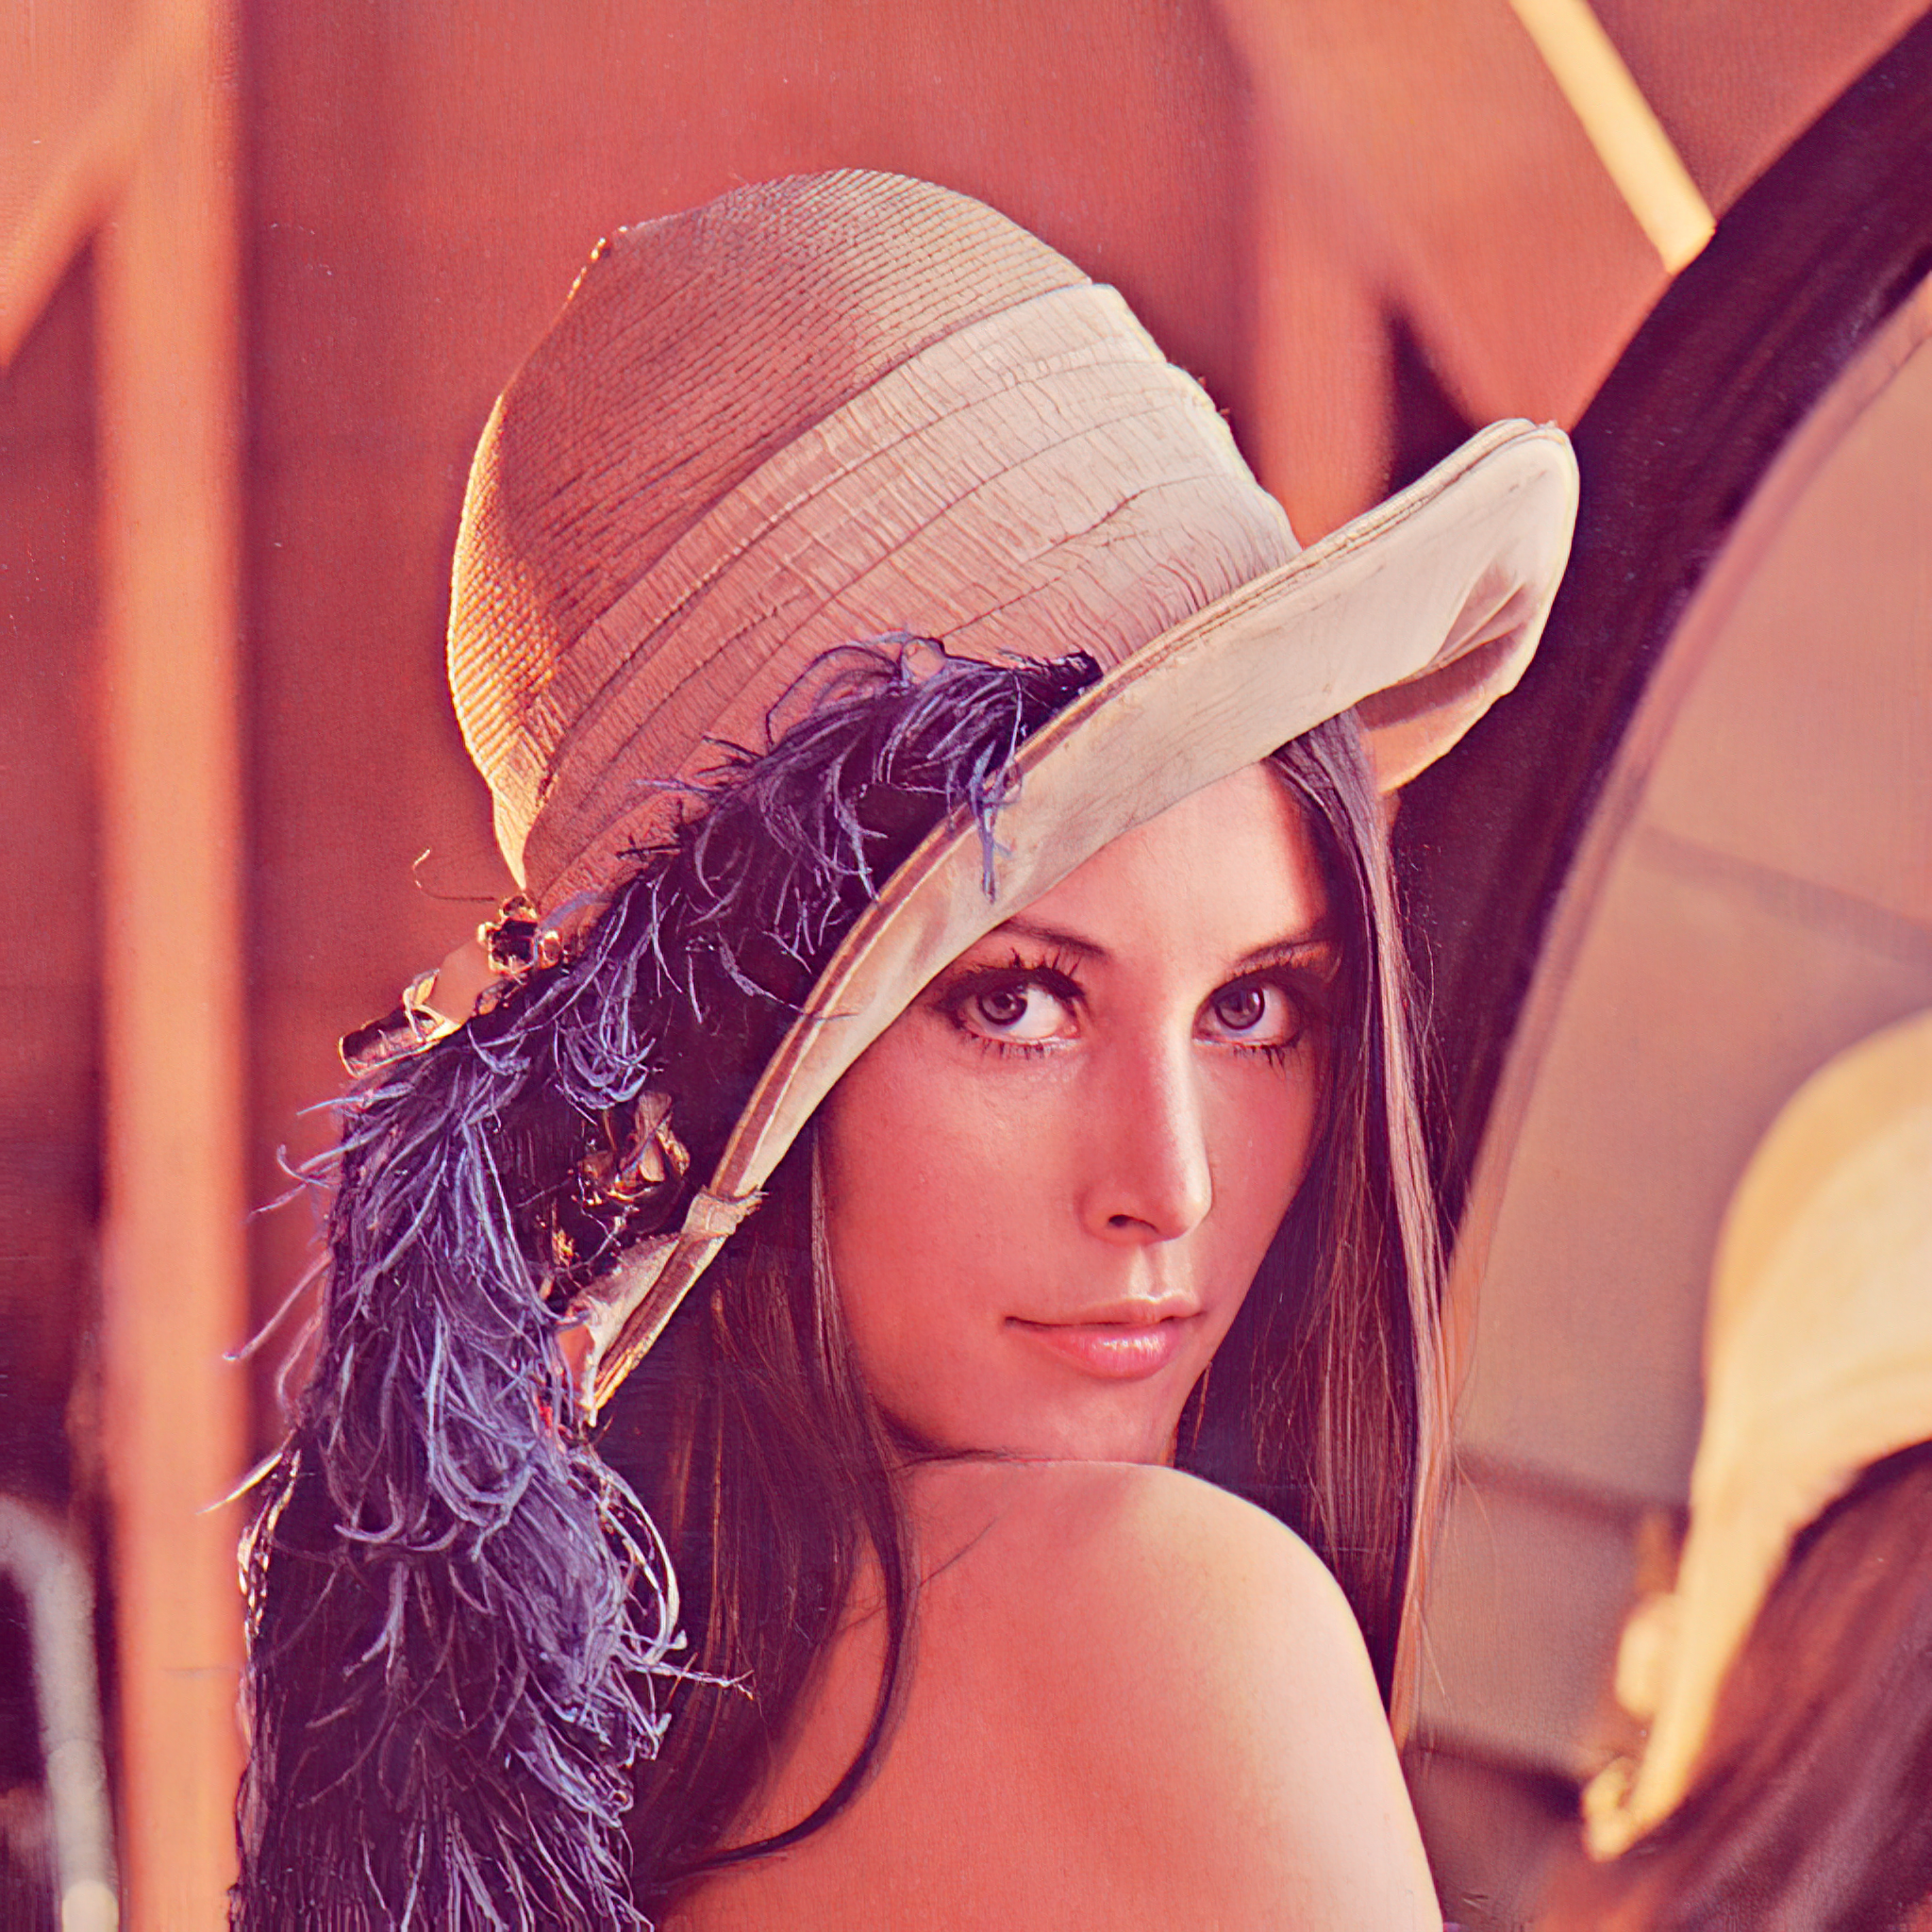
\includegraphics[width=0.5\textwidth]{Lenna}
%		\caption{Лена}
%%	\end{center}
%%	\vspace{5mm}
%%	\par
%\end{figure}

%\vspace{5mm}
%	\begin{center}
%		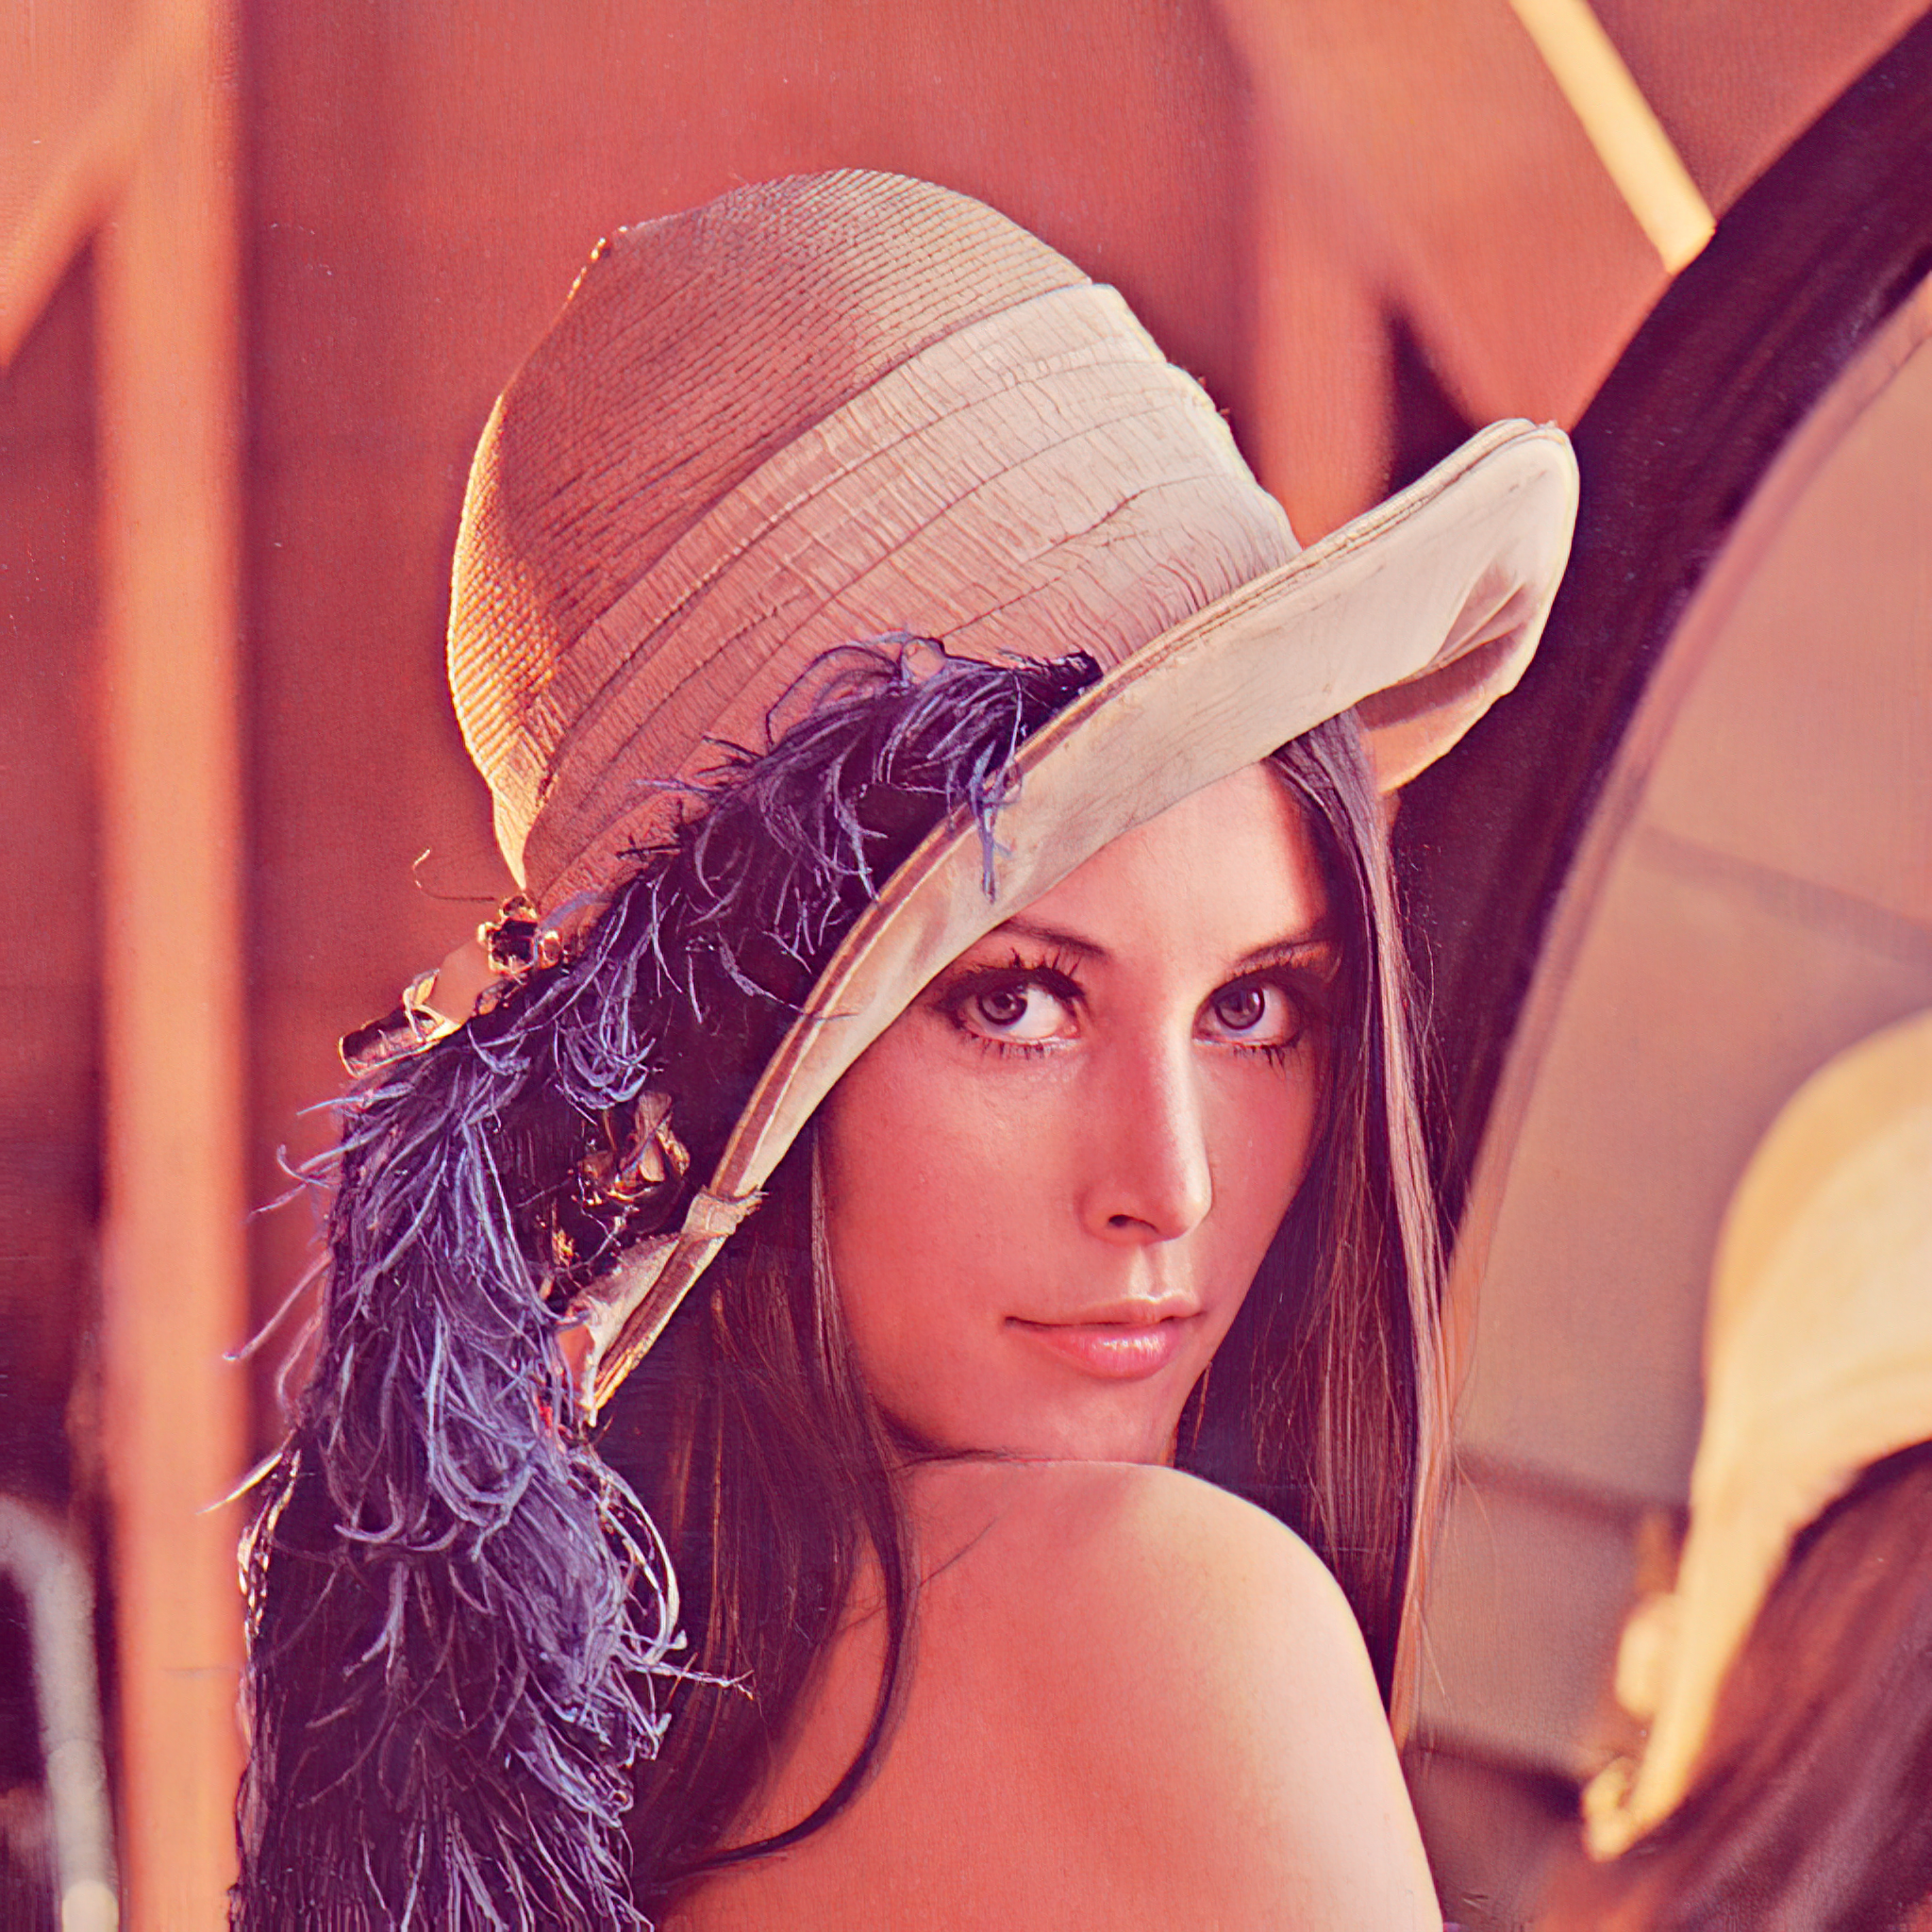
\includegraphics[width=0.5\textwidth]{Lenna}
%%		\caption{Лена}
%	\end{center}
%	\vspace{5mm}
%	\par



%\begin{figure}
%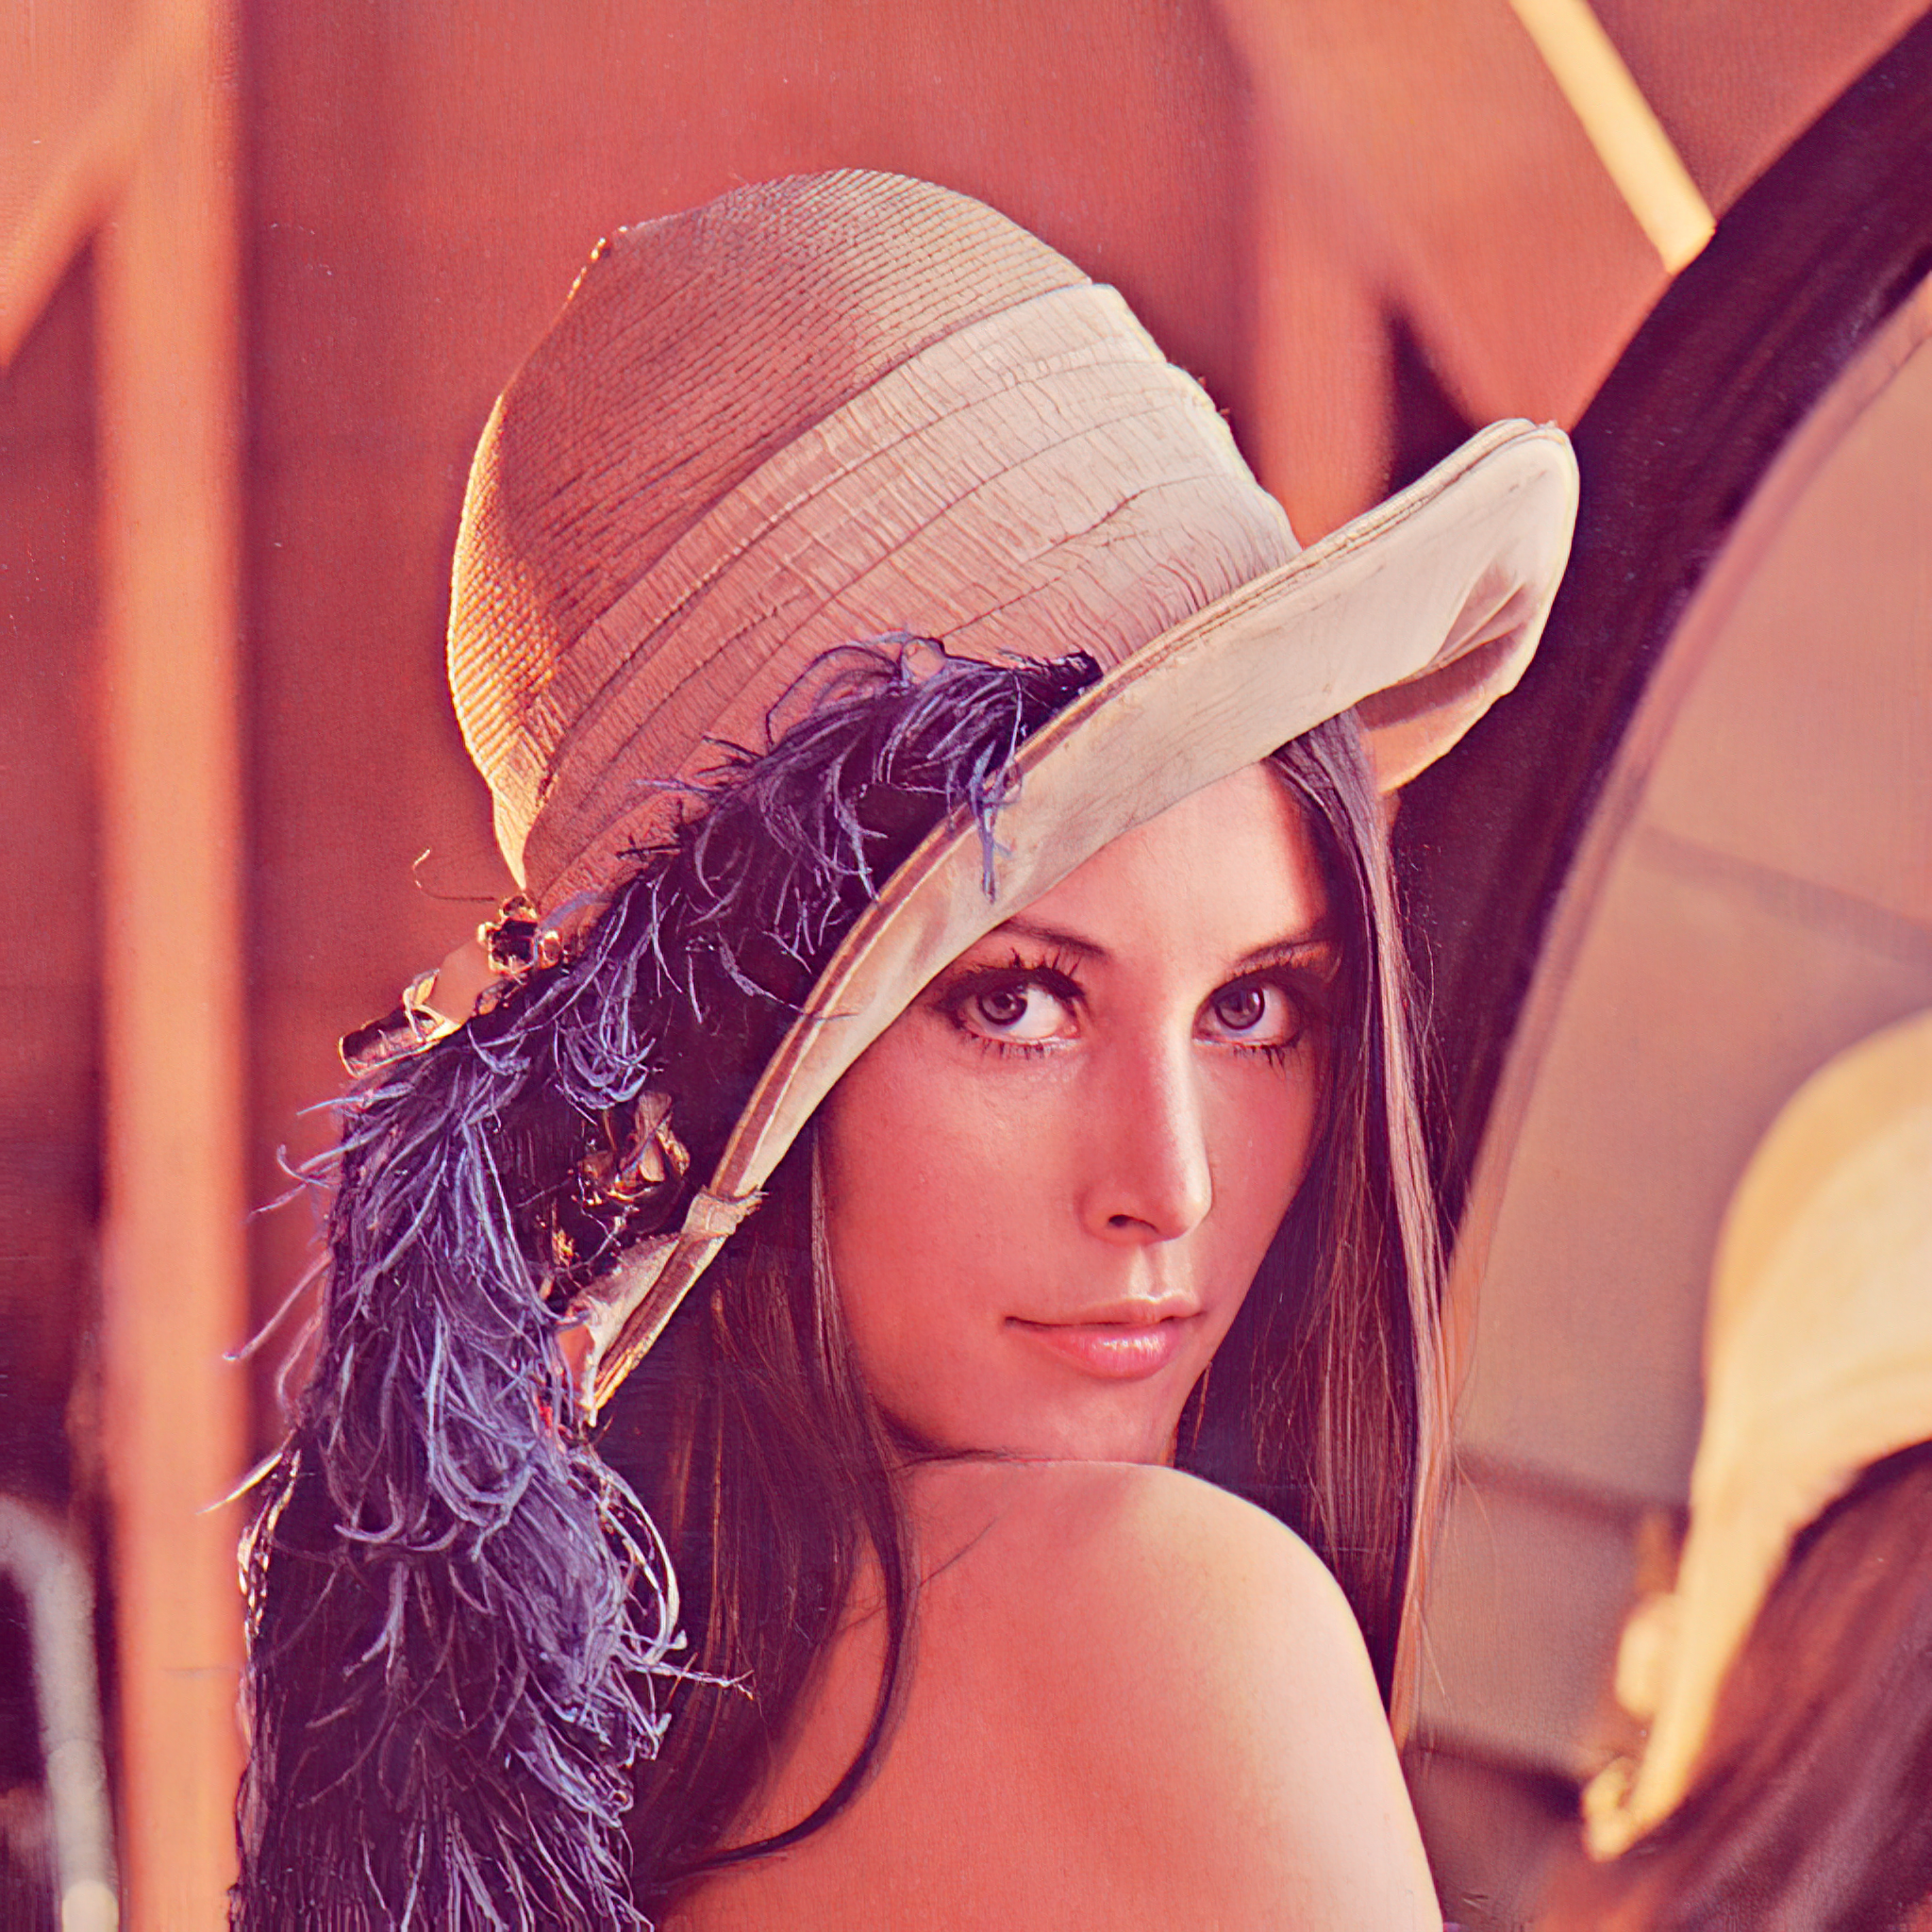
\includegraphics[width=8cm]{Lenna}
%\end{figure}
%\begin{figure}
%\image[0.5]{Lenna}
%\captionof{}{123}
%\caption{Caption}
%\label{fig:Лена}	
%\end{figure}
%
%\begin{figure}[h]
%	\centering
%	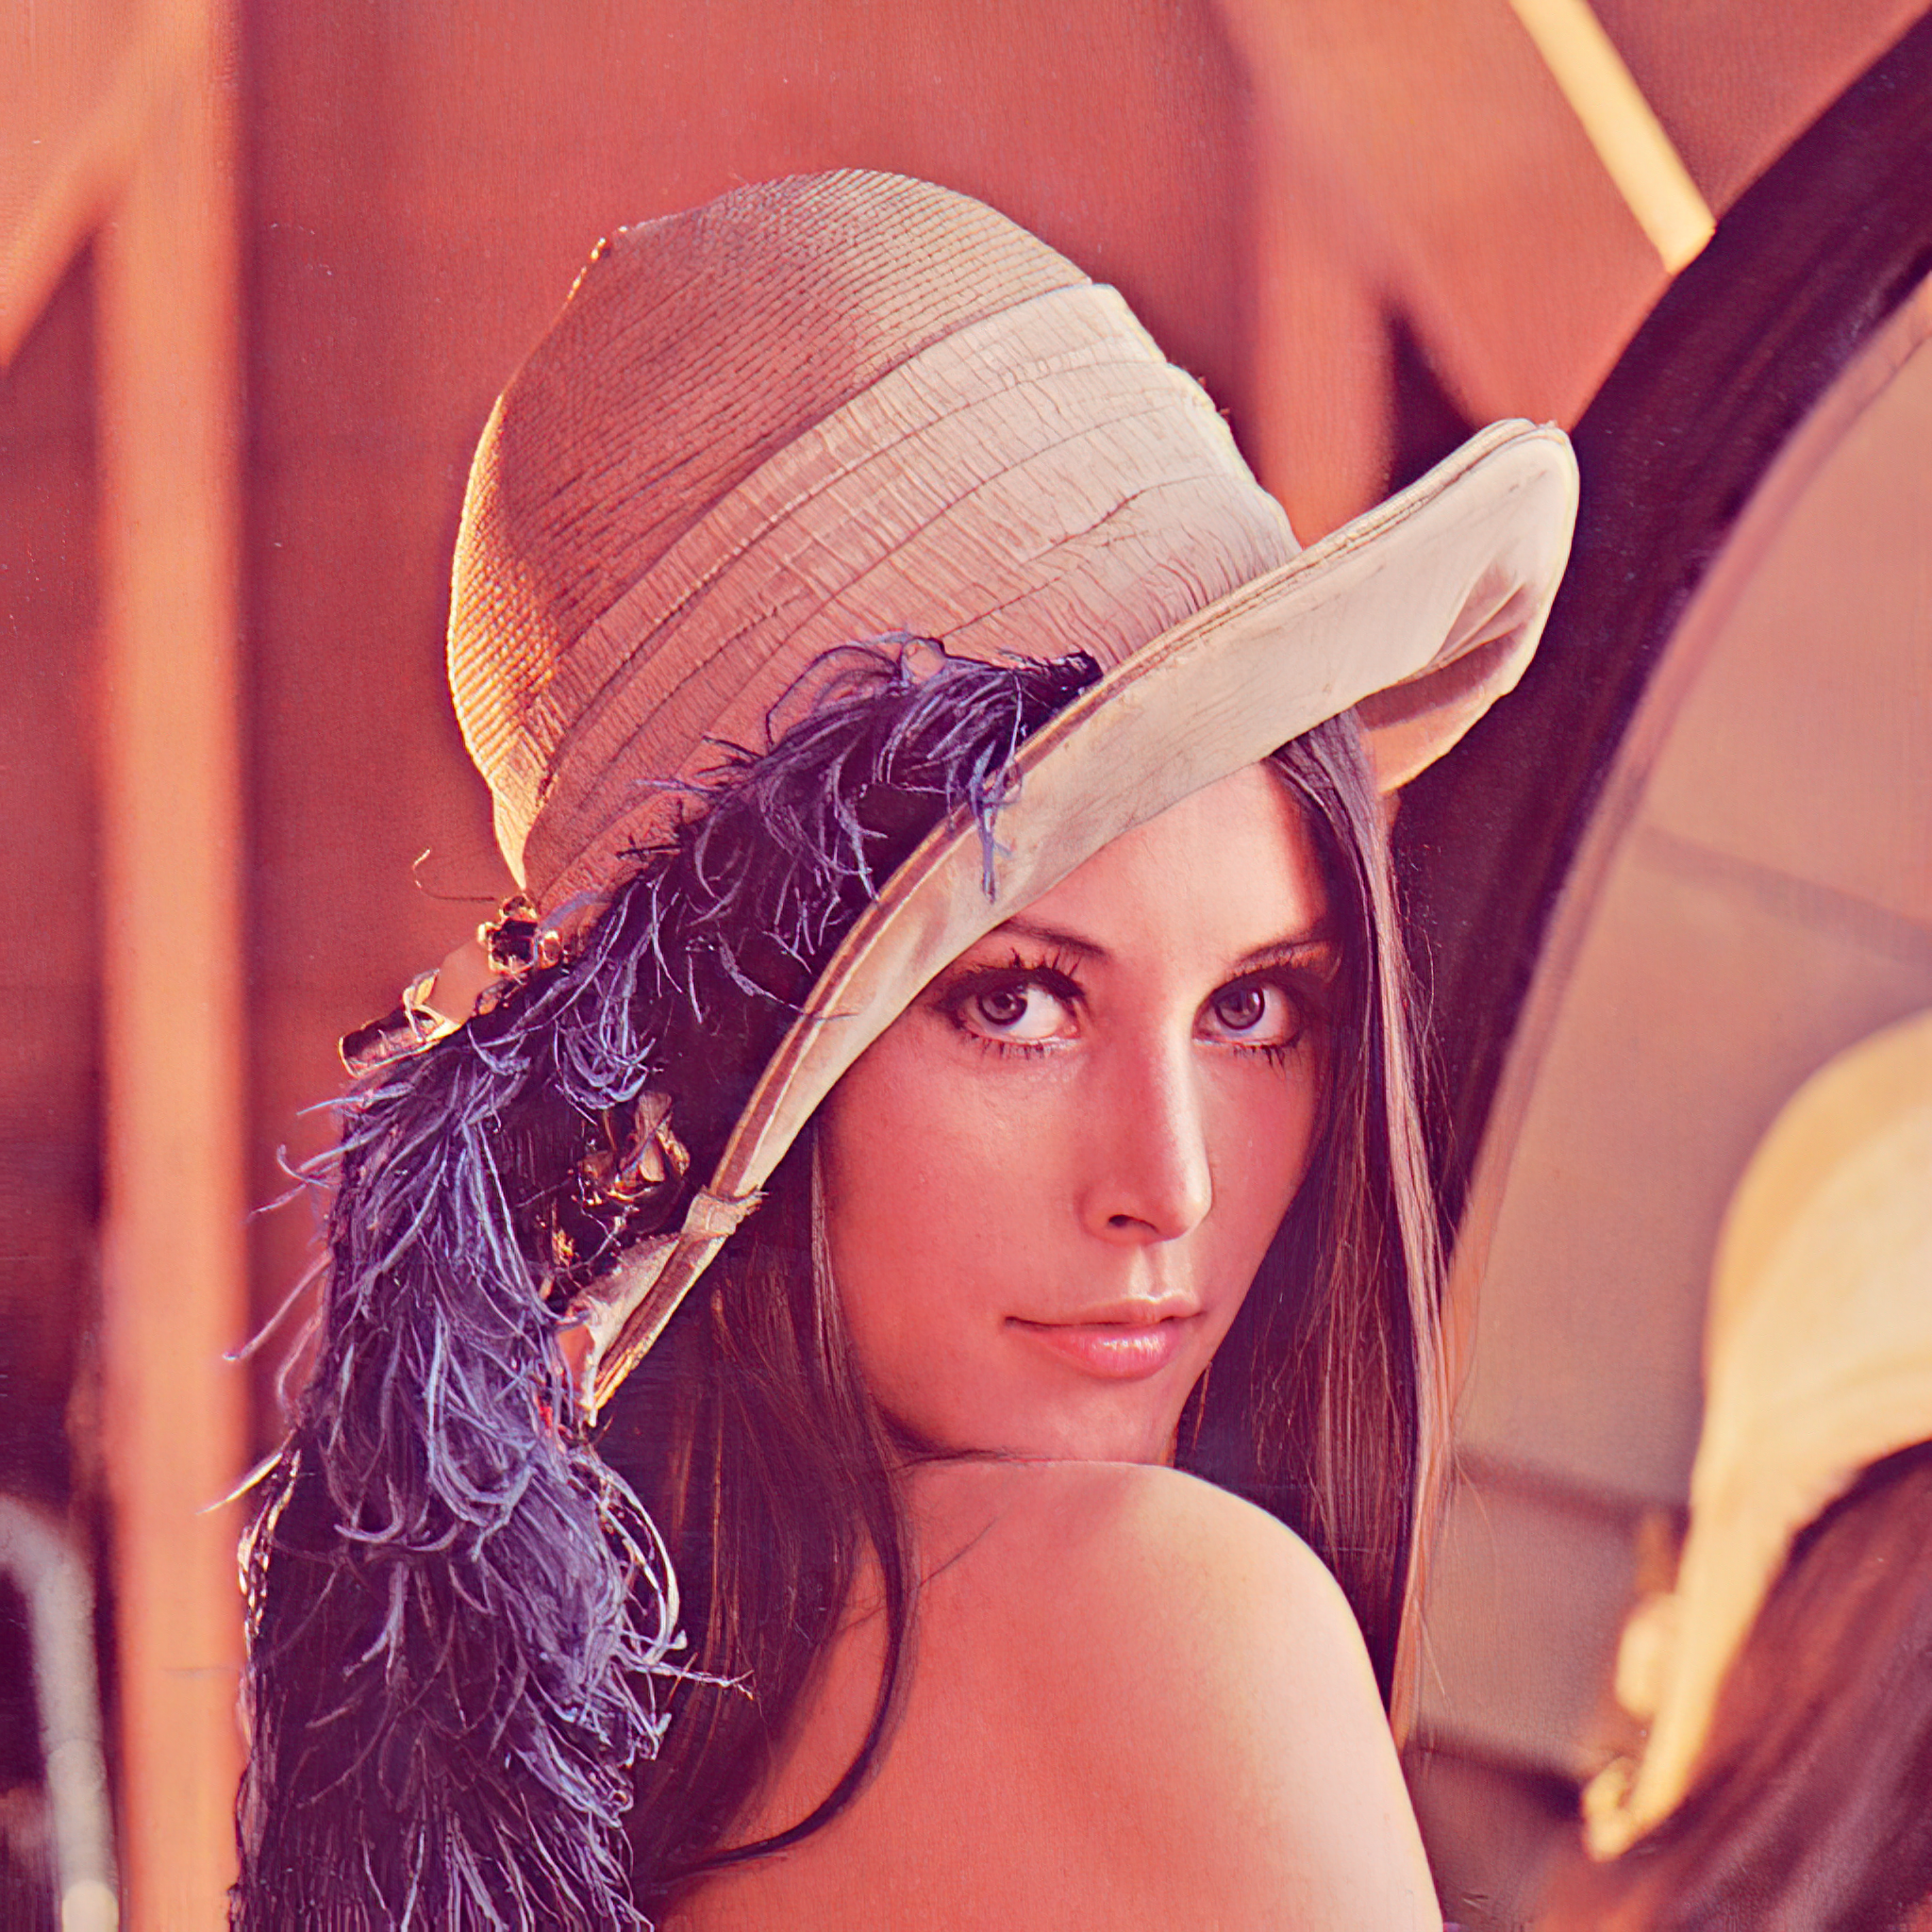
\includegraphics[width=\textwidth]{Lenna.png}
%%	\caption{Лена}
%%	\label{fig:Лена}
%\end{figure}
%
%

 
\newpage\section{Оформление формул}

В данном разделе приводится пример оформления формул по п.~2.4 ГОСТ~19.106 \cite{gost19106}.

\subsection{Простые примеры}

\paragraph{Формула без присвоения порядкового номера}

Пример формулы, вставляемой в тексте без присвоения порядкового номера: формула квадратного многочлена: $f(x) = ax^2 + bx + c$, где $a$\mdash первый (старший) коэффициент, $b$\mdash второй (средний) коэффициент, $c$\mdash свободный член.

\paragraph{Формула с автоприсвоением порядкового номера}
Пример формул с присвоением порядкового номера и без удаления пробелов:
\begin{align}
	x = y+a \label{eq:формула 1}\\
	z = a+x \label{eq:формула 2}
\end{align}
\noindent где: $x$\ndash коэффициент 1; \\
\indent $z$\ndash коэффициент 2;\\
\indent $y$\ndash параметр 1;\\
\indent $a$\ndash параметр 2.

Пример ссылки на формулу: см. формулу (\ref{eq:формула 1}).

Пример формул с присвоением порядкового номера и с удалением пробелов:
{\zerodisplayskips
	\begin{align}
	x = y+a \label{eq:формула 3}\\
	z = a+x \label{eq:формула 4}
	\end{align}
}%
\noindent где: $x$\ndash коэффициент 1; \\
\indent $z$\ndash коэффициент 2;\\
\indent $y$\ndash параметр 1;\\
\indent $a$\ndash параметр 2.

\newpage
\subsection{Примеры различных математических знаков и символов}

Приведем несколько примеров.

\begin{enumerate}
%%%%%%%%%%%%%%%%%%%%%%%%%%%%%%%%%%%%%%%%%%%%%%%%%%%%%%%%%%%%%%%%%%%%%%%%%%%%%%%	
\item индексы:
{\zerodisplayskips
	\begin{align}
	A_1, \label{eq:ф1}\\
	A_{\text{нижний индекс}}, \label{eq:ф2}\\
	A^{\text{верхний индекс(он же - степень)}}, \label{eq:ф3}\\
	A_{\text{нижний индекс}}^{\text{верхний индекс(он же - степень)}}. \label{eq:ф4}
	\end{align}	
}%
Отметим, что выравнивание в формулах (\ref{eq:ф1})\ndash (\ref{eq:ф4}) идёт по центру \textit{группы}.
%%%%%%%%%%%%%%%%%%%%%%%%%%%%%%%%%%%%%%%%%%%%%%%%%%%%%%%%%%%%%%%%%%%%%%%%%%%%%%%
\item некоторые греческие буквы с учетом русской традиции:	
{\zerodisplayskips
	\begin{equation}
	\alpha,\beta,\gamma,\phi,\epsilon,\theta. \label{eq:ф5}
	\end{equation}
}%
%%%%%%%%%%%%%%%%%%%%%%%%%%%%%%%%%%%%%%%%%%%%%%%%%%%%%%%%%%%%%%%%%%%%%%%%%%%%%%%
\item сумма, умножение, деление, дробь:
{\zerodisplayskips
	\begin{align}
	\text{сумма:}\quad & A+B=C, \label{eq:ф6}\\
	\text{умножение:}\quad & A\times B=C, \label{eq:ф7}\\
	\text{деление через косую черту:}\quad & A/B=C, \label{eq:ф8}\\
	\text{дробь (решение квадратного уравнения):}\quad & x_{1,2}=\frac{-b\pm\sqrt{b^2-4ac}}{2a}. \label{eq:ф9}\\
	\text{дробь (решение квадратного уравнения):}\quad & x_{1,2}=\frac{-b\pm\sqrt{b^2-4ac}}{2a}. \label{eq:ф99}
	\end{align}
}%

Знак <<\&>> внутри формулы и конструкции \verb=\begin{align}...\end{align}= вызывает выравнивание по этому символу. 

Обратите внимание, повторная вставка формулы (\ref{eq:ф99}) вызывает автоматическое выравнивание по высоте.
%%%%%%%%%%%%%%%%%%%%%%%%%%%%%%%%%%%%%%%%%%%%%%%%%%%%%%%%%%%%%%%%%%%%%%%%%%%%%%
\item производная и интеграл:
{\zerodisplayskips
	\begin{equation}	
	f’\quad f’’\quad
	\dot{f}\quad \ddot{f} \quad
	\frac{d f}{d x}\quad
	\frac{\partial f}{\partial x}
	\int_0^{\infty}\quad
	\int\limits_0^{\infty}.\quad
	\label{eq:ф10}
	\end{equation}
}%
%%%%%%%%%%%%%%%%%%%%%%%%%%%%%%%%%%%%%%%%%%%%%%%%%%%%%%%%%%%%%%%%%%%%%%%%%%%%%%
\item знак суммы:
{\zerodisplayskips
	\begin{equation}	
	\sum_{i=1}^n a_i,\quad
	\sum\nolimits_{i=1}^n b_i\quad
	\label{eq:ф11}
	\end{equation}
}
%%%%%%%%%%%%%%%%%%%%%%%%%%%%%%%%%%%%%%%%%%%%%%%%%%%%%%%%%%%%%%%%%%%%%%%%%%%%%%%
\item перенос формул вручную c указанием места разделения и команды \verb=split=:
{\zerodisplayskips
	\begin{equation}	
	\begin{split}
	x&=1000+1100+{}\\
	 &+1200+1300.
	\end{split}
	\label{eq:ф12}
	\end{equation}
}
%%%%%%%%%%%%%%%%%%%%%%%%%%%%%%%%%%%%%%%%%%%%%%%%%%%%%%%%%%%%%%%%%%%%%%%%%%%%%%%
\item системы уравнений с фигурной скобкой:
{%\zerodisplayskips
	\begin{equation}	
	\left\{
	\begin{aligned}
	x^2+y^2&=7\\
	x+y & = 3.\\
	\end{aligned}
	\right.
	\end{equation}
}
%%%%%%%%%%%%%%%%%%%%%%%%%%%%%%%%%%%%%%%%%%%%%%%%%%%%%%%%%%%%%%%%%%%%%%%%%%%%%%
\item длина волны через частоту:
{\zerodisplayskips
	\begin{equation}	
	\lambda=C/(Fr \times 10^3),
	\end{equation}
}
%%%%%%%%%%%%%%%%%%%%%%%%%%%%%%%%%%%%%%%%%%%%%%%%%%%%%%%%%%%%%%%%%%%%%%%%%%%%%%
\item пример очень длинной формула с переносом:
{\zerodisplayskips
	\begin{equation}
	\begin{split}	
	Vf_i&=X.V_i\times 0.5 \times (cos((X.K_i - AzEndR_i)\times DgToRd) +{}\\
	    &+cos((X.K_i - AzEndT_i)\times DgToRd).
	\label{eq:ф14}
	\end{split}
	\end{equation}
}
%%%%%%%%%%%%%%%%%%%%%%%%%%%%%%%%%%%%%%%%%%%%%%%%%%%%%%%%%%%%%%%%%%%%%%%%%%%%%%
\item пример автовыбора высоты скобок путем использования команд \verb=\left= и \verb=\right= соответственно:
{\zerodisplayskips
	\begin{equation}
	f(x)=1+\left(\frac{1}{1-x^{2}}
	\right)^3
	\end{equation}
}
%%%%%%%%%%%%%%%%%%%%%%%%%%%%%%%%%%%%%%%%%%%%%%%%%%%%%%%%%%%%%%%%%%%%%%%%%%%%%%
\item пример многоэтажной дроби:
{\zerodisplayskips
	\begin{equation}
	X=\frac{\ln\left(\cfrac{A}{B}\right)\times \ln\left(\cfrac{C}{D}\right)}{\ln\left(\cfrac{E}{F} \right)\times \ln\left(\cfrac{G}{H} \right)}
	\end{equation}
}
%%%%%%%%
\end{enumerate}	


 
\section{Оформление таблиц}

В данном разделе приводится пример иерархии вложенности по п.~2.6 ГОСТ~19.106 \cite{gost19106}.

Оформление всегда следует вести при помощи класса \lstinline|longtable|, поскольку это дает возможность переноса длинной таблицы на следующую страницу.

\subsection{Простая маленькая таблица}

Простой пример маленькой таблицы c маленькими колонками, выровненными по центру, без каких-либо переполнений.

% Всегда вставлять параметр [с] после longtable - выравнивание по центру страницы
\begin{longtable}[c]{| >{\centering}m{25mm} | >{\centering}m{25mm} | >{\centering}m{50mm} |}
	\caption{Пример маленькой таблицы\hspace{25cm}} % \hspace{25cm} - хак, для того чтобы было выровнено по левому краю, иначе без головной боли не получилось
	\label{t:tab0} \\		
	\hline % горизонтальная линия
	колонка 1 & колонка 2 & колонка 3 \tabularnewline
	\hhline{|=|=|=|} % горизонтальная двойная линия
	111 & 222 & 333
	\tabularnewline\hline % горизонтальная линия
\end{longtable}

\subsection{Широкая таблица с длинными заголовками колонок}

Пример таблицы с длинными заголовками колонок

\begin{longtable}[c]{| >{\raggedright}m{55mm} | >{\centering}m{55mm} | >{\raggedleft}m{55mm} |}
	\caption{Пример таблицы c возможно очень длинным заголовком, который будет перенесен на вторую строчку\hspace{25cm}} % \hspace{25cm} - хак, для того чтобы было выровнено по левому краю, иначе без головной боли не получилось
	\label{t:tab1} \\		
	\hline % горизонтальная линия
	колонка 1 с очень длинным заголовком, просто капец каким длинным & колонка 2 по центру & колонка 3 по правому краю \tabularnewline
	\hhline{|=|=|=|} % горизонтальная двойная линия
	Содержание колонки 1 & Содержание колонки 2 & Содержание колонки 3, возможно очень длинное содержание, которое нормально отображается с переносом по словам
	\tabularnewline\hline % горизонтальная линия
\end{longtable}

Пример оформления ссылки на таблицу: см.~табл.~\ref{t:tab1}.

\newpage
\subsection{Часто встречающая в документации таблица}

Пример таблицы, часто встречающийся в программной документации:

\begin{longtable}[c]{| >{\centering}m{15mm} | >{\raggedright}m{50mm} | >{\raggedright}m{20mm} | >{\centering}m{20mm} | >{\raggedright}m{30mm} | >{\centering}m{18mm} |}
	%----------------------- преамбула ---------------------	
	\caption{Пример таблицы\hspace{25cm}}
	\label{t:tab2} \\
	\hline
	Номер слова & Наименование информации & Усл.~об. & Размерн. & Пределы изменения & Примеч. \tabularnewline
%	\hline
	\hhline{|=|=|=|=|=|=|}
	\endfirsthead % Конец заголовка на 1 странице
%	\hline
	\multicolumn{6}{r}{\tabletextsize продолжение табл.\thetable} \\ 
	\hline
	Номер слова & Наименование информации & Усл.~об. & Размерн. & Пределы изменения & Примеч. \tabularnewline
%	\hline
	\hhline{|=|=|=|=|=|=|}
	\endhead
	\hline
	\multicolumn{6}{r}{\tabletextsize см. далее}
	\endfoot
	\hline
	\endlastfoot	
	%------------------- табличные данные ------------------

	1 & Контрольное слово & CW\textunderscore & б/р & \ndash & uint \tabularnewline\hline
	2 & Контрольное слово & CW\textunderscore & б/р & \ndash & uint \tabularnewline\hline
	3 & Контрольное слово & CW\textunderscore & б/р & \ndash & uint \tabularnewline\hline
	4 & Контрольное слово & CW\textunderscore & б/р & \ndash & uint \tabularnewline\hline
	5 & Контрольное слово & CW\textunderscore & б/р & \ndash & uint \tabularnewline\hline	
	6 & Контрольное слово & CW\textunderscore & б/р & \ndash & uint \tabularnewline\hline	
	7 & Контрольное слово & CW\textunderscore & б/р & \ndash & uint \tabularnewline\hline	
	8 & Контрольное слово & CW\textunderscore & б/р & \ndash & uint \tabularnewline\hline	
%
%	\newpage % Принудительный перенос на новую страницу
%
	9 & Контрольное слово & CW\textunderscore & б/р & \ndash & uint \tabularnewline\hline	
	10 & Контрольное слово & CW\textunderscore & б/р & \ndash & uint \tabularnewline\hline	
	11 & Контрольное слово & CW\textunderscore & б/р & \ndash & uint \tabularnewline\hline	
	12 & Контрольное слово & CW\textunderscore & б/р & \ndash & uint \tabularnewline\hline	
	13 & Контрольное слово & CW\textunderscore & б/р & \ndash & uint \tabularnewline\hline	
	14 & Контрольное слово & CW\textunderscore & б/р & \ndash & uint \tabularnewline\hline	
	15 & Контрольное слово & CW\textunderscore & б/р & \ndash & uint \tabularnewline\hline	
	16 & Контрольное слово & CW\textunderscore & б/р & \ndash & uint \tabularnewline\hline	
	17 & Контрольное слово & CW\textunderscore & б/р & \ndash & uint \tabularnewline\hline	
	18 & Контрольное слово & CW\textunderscore & б/р & \ndash & uint \tabularnewline\hline	
	19 & Контрольное слово & CW\textunderscore & б/р & \ndash & uint \tabularnewline\hline	
	20 & Контрольное слово & CW\textunderscore & б/р & \ndash & uint \tabularnewline\hline		
\end{longtable}

Пример оформления ссылки на таблицу: см.~табл.~\ref{t:tab2}.
 
\include{оформление_листингов}
\bibliography{список_литературы}
\begin{terms}
\term{Latex}{язык верстки текста}
\end{terms}
\begin{abbreviations}
\abbr{ГОСТ}{государственный стандарт}
\abbr{ЕСПД}{единая система программной документации}
\end{abbreviations}
\include{приложение_1}
\include{приложение_2}
}
\end{document}
